
\section{Problemformulering}
At designe og fremstille et éndimensionelt vognmonteret omvendt pendul, der ved hjælp af regulering skal kunne fastholde en forudbestemt vinkel af pendulet, samt at kunne kompensere for udefrakommende påvirkninger. 

\subsection{Formål}
Formålet med projektet er, at forene de opnåede fagligheder fra undervisningen på 3. semester. 
Alle fag fra undervisningen indgår i projektet, og er henholdsvis elektronik, elektromagnetisme, regulering, kredsløbsteknik og matematik.
Det er dermed ønskeligt, at eftervise teorien med praksis. 


\subsection{Krav til rapporten stillet i projektoplæg}
Semestertema: Måling og generering af elektromagnetiske felter kombineret med analog signalbehandling.
\begin{itemize}
\item Der skal udføres et projekt i overensstemmelse med semestertemaet.
\item Projektet skal indeholde fagligheder fra alle teorifagene. Fra elektrofysikken skal
magnetiske felter behandles.
\item Der skal foretages en grundig problemanalyse, der munder ud i en klar og entydig
problemformulering.
\item Produktet skal i videst mulig omfang baseres på lagerførte varer.
\end{itemize}

\subsection{Selvvalgte krav til projektet} \label{afs:kravspecifikation}
Udover de på forhånd stillede projektkrav, er der blevet foretaget yderligere selvvalgte krav, som fremgår herunder.
\begin{itemize}
\item Pendulet skal altid starte i ligevægtsposition, og må kun påvirkes små udefrakommende krafter.
\item Systemet skal kunne drives af to batterier.
\item Sensoren skal være induktiv.
\end{itemize}

\subsection{Problemstilling}
Følgende problemstillinger ønskes besvaret:
\begin{itemize}
\item Hvordan finder mand spændingsforholdet mellem 2 spoler?
\item Hvordan udregnes magnetfeltet i en spole?
\end{itemize}

\subsection{Projektafgrænsning}
Følgende medtages ikke i rapporten og afgrænser projektarbejdet:
\begin{itemize}
\item Systemet skal kun virke i én retning (dimension)
\item Der ses bort fra den fysiske beskrivelse af elektromotoren.
\item Vogn samt tilhørende motor, hjul og gearing overtages fra tidligere projekt.
\end{itemize}

\section{Løsningsmodel}
\begin{figure}[h!]
	\centering
	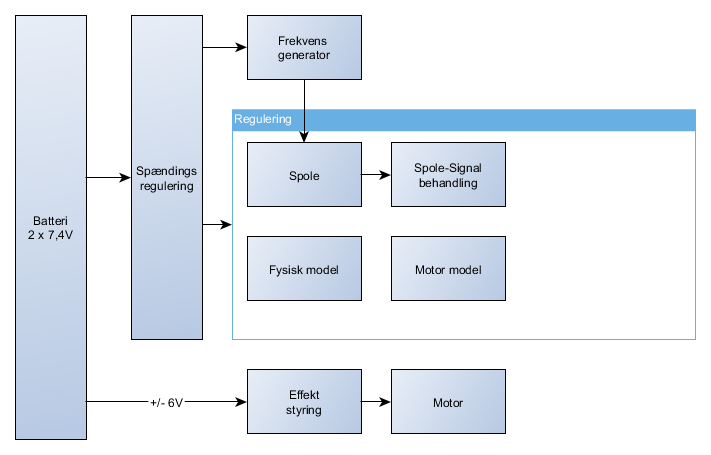
\includegraphics[width=.9\textwidth]{diagram/blokdiagram1.png}
	\caption{System blokdiagram.}
	\label{fig:blockdiagram1}
\end{figure}
\FloatBlock

\husk{JJ}{Del diagram af system og signalvej ?}


\section{Læsevejledning}
Denne rapports struktur er delt op i hovedsektioner og undersektioner.
Rapporten er opbygget taksonomisk. 
Derudover indeholder hvert kapitel en delkonklusion og opsummering af kapitlets gennemgang.
For at få mest ud af denne rapport, anbefales at læse fra start til slut i punktform, da opbygningen er baseret på systemets signalvej.
Man vil få en forståelse for hvordan hele systemet er bygget op, både teoretisk og praktisk. 


\section{Arbejdsmetode}
Noter til arbejdsmetoden.
Disse krav er estimeret løbende i projektets fremskriden.
\begin{itemize}
	\item Iterativ planlægning
	\item ugentlige status møder hvor der opsummeres
	\item fleksibel opgave styring, for maksimal udnyttelse af ressourcer 
	\item To-Do lister
\end{itemize}